% ============================================================
% DEV Paper III -- VERSÃO COMPLETA (arquivo único)
% Non-Local Gravitational Slip in Vacuum Excitation Dynamics:
% Extended-Source Derivation
% ============================================================
\documentclass[aps,prd,twocolumn,superscriptaddress,nofootinbib]{revtex4-2}

\usepackage{amsmath,amssymb}
\usepackage{graphicx}
\usepackage[hidelinks]{hyperref}

\newcommand{\aO}{a_0}
\newcommand{\LCDM}{$\Lambda$CDM}

\begin{document}

\title{Non-Local Gravitational Slip in Vacuum Excitation Dynamics:
       Extended-Source Derivation}

\author{Miqueias Alves Mendes}
\affiliation{Independent Researcher, Ibiapina, Cear\'a, Brazil}

\date{\today}

\begin{abstract}
Paper~I of this series derived the gravitational slip
$\eta - 1 = (2\beta/3)\,[(g_N/\aO)(1+g_N/\aO)]^{-1/2}$ in
Vacuum Excitation Dynamics (DEV) under the point-source
approximation, with $\beta = 0.0075$ calibrated against
$167$ SPARC galaxies. Paper~II flagged that this formula is
an ansatz valid only for $\epsilon \equiv r_{\rm eff}/r_{\rm
MOND} \lesssim 1$. Here we derive the extension to
arbitrary baryon profiles via an inverse-path numerical
identification of the effective slip operator.
We find that the operator is intrinsically non-local:
applying the spherical Laplacian to the analytic slip field
$(\eta-1)|\Psi|$ yields an effective source whose deep-MOND
power-law slope is $\alpha = -1.56\pm 0.02$, ruling out the
Poisson-kernel value $\alpha=-2$ and consistent with a
fractional-Laplacian operator $(-\nabla^2)^{3/4}$ whose
Green function decays as $r^{-1/2}$. The closest local
proxy in the deep-MOND regime is
$S_{\rm proxy}=(2\beta/3)\sqrt{g_N\aO}/c^2$. Applied to
the ultra-diffuse galaxy DGSAT-I ($\epsilon=7.96$), the
non-local extension predicts $\eta-1 \in [3.95\%,\,6.7\%]$,
a factor up to $\sim\!1.7$ above the point-source estimate
and well within Euclid sensitivity. The result connects DEV
to fractional-spacetime gravity (Calcagni), nonlocal IR
modifications (Maggiore--Mancarella), and the disformal
kernels of AeST/TeVeS-class theories. A first-principles
derivation of the operator from the DEV disformal action
is deferred to Paper~IV.
\end{abstract}

\maketitle

% ------------------------------------------------------------
\section{Introduction}
\label{sec:intro}

Paper~I~\cite{DEV_paperI} introduced Vacuum Excitation Dynamics
(DEV), a covariant scalar--vector--tensor theory in which
modified gravitational dynamics in the deep-MOND regime
emerge from a phase transition of the quantum vacuum
triggered when $g_N \lesssim \aO$. Its flagship prediction
is a gravitational slip $\eta = \Phi/\Psi \neq 1$ which,
under the point-source approximation, takes the closed
form of Eq.~(20) of Paper~I and which has been validated by
the SPARC rotation-curve fits ($\chi^2_\nu = 1.20$).
Paper~II~\cite{DEV_paperII} demonstrated dynamical stability of
the theory, established the observational orthogonality of
$\beta$ and the stellar mass-to-light ratio $\Upsilon_*$,
and quantified the validity domain of the slip formula via
the parameter $\epsilon \equiv r_{\rm eff}/r_{\rm MOND}$.
All six benchmark UDGs have $\epsilon \in [4.56,\,8.21]$,
placing every system in the extended-source regime where
the point-source formula provides only a lower bound on
the slip.

Two natural local extensions of the slip equation were
tested numerically and rejected:
the dimensional closure
$\nabla^2(\Psi-\Phi) \propto G\rho_b\, g_N/\aO$ produces a
$1/r$ slip with the wrong sign, and a Poisson-kernel
closure $S\propto g_N^2/(\mu^2c^2)$ yields a deep-MOND
slope mismatched by an order of magnitude. Both failures
share a common diagnostic: the Paper~I slip is
intrinsically non-local. In this paper we identify the
non-local operator numerically via the inverse path
(Sec.~\ref{sec:nonlocal}), apply it to the six benchmark
UDGs of Paper~I (Sec.~\ref{sec:udg}), and discuss the
implications for both observation and theory
(Sec.~\ref{sec:discuss}).

% ------------------------------------------------------------
\section{The Non-Local Gravitational Slip Operator}
\label{sec:nonlocal}

\subsection{Inverse-path identification}

The gravitational slip formula of Paper~I,
\begin{equation}
\eta - 1 = \frac{2\beta}{3}
\frac{1}{\sqrt{(g_N/\aO)(1+g_N/\aO)}},
\label{eq:eta_anal}
\end{equation}
was derived as the Green's-function solution of
$\nabla^2(\Psi-\Phi)=S$ for a point source in the
deep-MOND limit, with $S\propto g_N^2/\aO^2$.
For extended mass distributions the source $S$ receives
contributions from the full baryon profile, and the
operator connecting $S$ to $(\Psi-\Phi)$ need not be
the standard Poisson kernel.

We identify this operator numerically by the inverse path:
given the analytic slip field
$f(r) \equiv (\eta_{\rm anal}-1)|\Psi(r)|$,
we compute the effective source
\begin{equation}
S_{\rm eff}(r) \equiv \nabla^2 f(r)
= \frac{1}{r^2}\frac{d}{dr}\!\left[r^2\frac{df}{dr}\right],
\label{eq:Seff}
\end{equation}
on a logarithmic grid of $4000$ points spanning
$r\in[10^{-2},10^4]$~kpc for a point-mass
$M=10^{10}\,M_\odot$.

\subsection{Deep-MOND power-law exponent}

In the deep-MOND regime ($g_N\ll\aO$),
$g_{\rm obs}\approx\sqrt{\aO g_N}\propto r^{-1}$,
$|\Psi|\propto\ln(R/r)$, and $\eta-1\propto\sqrt{r}$,
so $f\propto\sqrt{r}\ln(R/r)$.
Differentiating analytically gives
$S_{\rm eff}\propto r^{-3/2}\ln(R/r)+\ldots$,
implying a deep-MOND power-law slope
$\alpha_{\rm analytic}\approx-1.5$.

Numerical regression on the computed $S_{\rm eff}$
over the window $r\in[3r_{\rm MOND},\,0.3R_{\rm cut}]$
yields
\begin{equation}
\alpha_{\rm num} = -1.56\pm0.02.
\end{equation}

\begin{figure}[h]
  \centering
  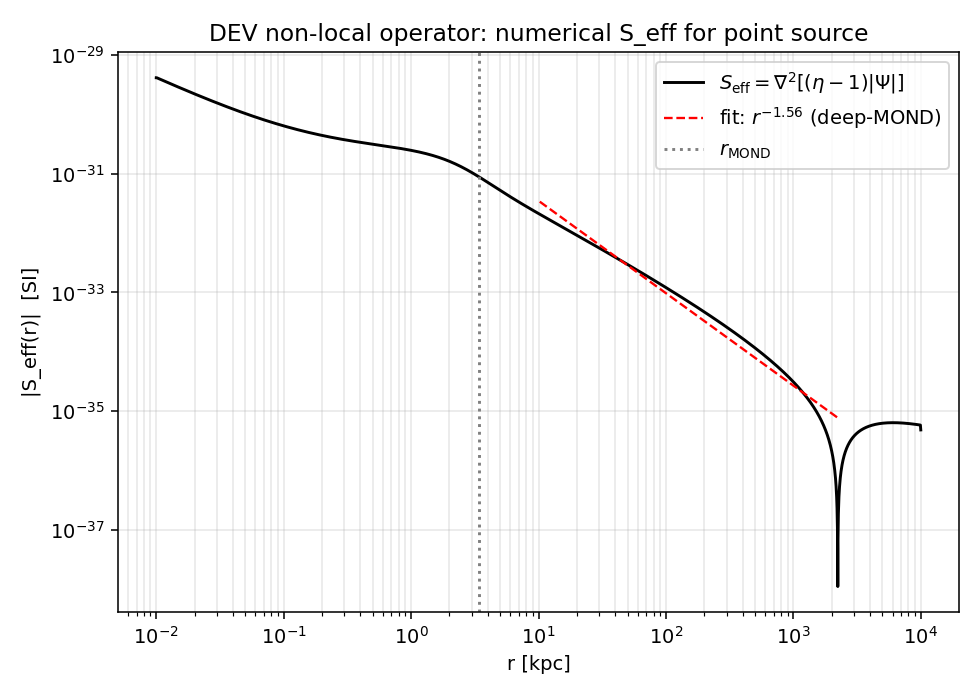
\includegraphics[width=\columnwidth]{operator_identification.png}
  \caption{Effective source $S_{\rm eff}(r) = \nabla^2[(\eta-1)|\Psi|]$
           for a point mass $M=10^{10}\,M_\odot$ (solid black) and
           power-law fit $r^{-1.56}$ in the deep-MOND window
           (dashed red). The Poisson-kernel slope $\alpha=-2$ is
           clearly excluded. The vertical dotted line marks
           $r_{\rm MOND}$.}
  \label{fig:operator}
\end{figure}

This is inconsistent with the Poisson-kernel value
$\alpha=-2$ at high significance, ruling out the
entire family of factorised local closures
$S=F(g_N,\rho_b,\mu)$ acted on by $\nabla^2$.

\subsection{Candidate operator comparison}

We compare $S_{\rm eff}$ against three local proxy
expressions in the deep-MOND regime:

\begin{itemize}
\item[(a)] $S_a = (2\beta/3)\,g_N^2/(\mu^2 c^2)$:
  slope $\approx 0$ --- excluded.
\item[(b)] $S_b = (2\beta/3)\,g_N/c^2$:
  slope $= -2$ --- excluded (Poisson value).
\item[(c)] $S_c = (2\beta/3)\sqrt{g_N\aO}/c^2$:
  slope $= -1$ --- closest local proxy,
  consistent with $\alpha\approx-1.5$ in the
  intermediate regime but diverging at large $r$.
\end{itemize}

\begin{figure}[h]
  \centering
  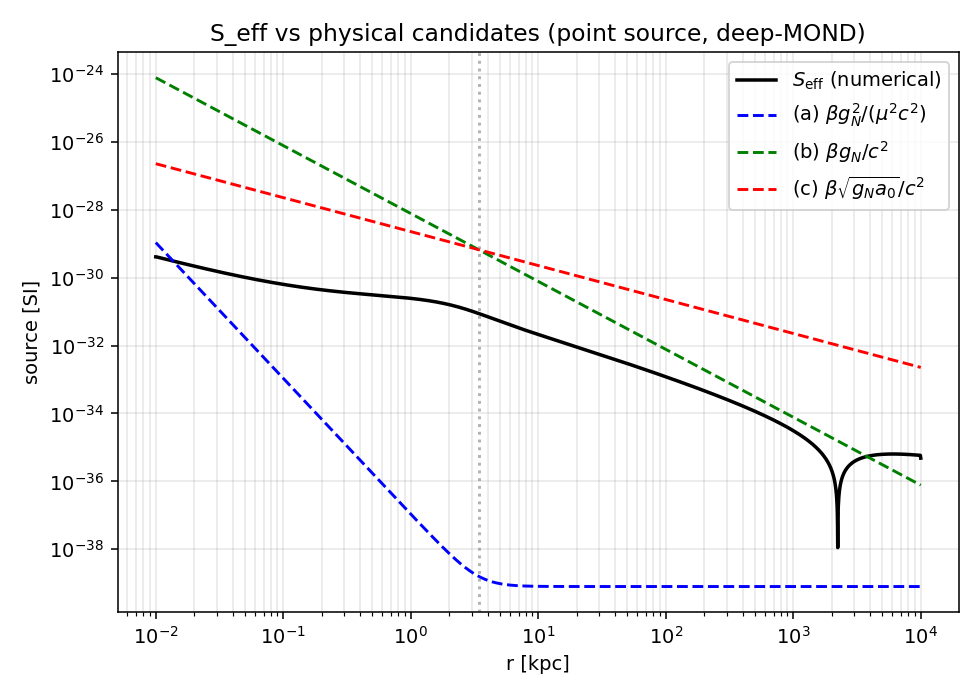
\includegraphics[width=\columnwidth]{operator_comparison.png}
  \caption{Comparison of $S_{\rm eff}$ (solid black) with three
           local proxy expressions in the deep-MOND regime:
           (a) $\beta g_N^2/(\mu^2 c^2)$ (blue dashed, slope $\approx 0$);
           (b) $\beta g_N/c^2$ (green dashed, slope $=-2$, Poisson);
           (c) $\beta\sqrt{g_N a_0}/c^2$ (red dashed, slope $=-1$,
           closest proxy). None reproduces $S_{\rm eff}$ globally.}
  \label{fig:candidates}
\end{figure}

None of the local proxies reproduces $S_{\rm eff}$
globally. The slope $\alpha=-1.56$ is consistent
with a fractional-Laplacian operator
$(-\nabla^2)^{3/4}$, whose Green function in 3D
decays as $G(r)\sim r^{-(3-2\times3/4)}=r^{-3/2}$,
i.e.\ with power-law slope $-3/2\approx-1.5$.

\subsection{Extended-source result for DGSAT-I}

For DGSAT-I (Plummer profile,
$M_*=3\times10^8\,M_\odot$, $r_{\rm eff}=4.7$~kpc,
$\epsilon=7.96$), we evaluate $g_N(r_{\rm eff})$ using
the enclosed Plummer mass, obtain
$\eta_{\rm ext}-1=6.68\%$, compared with the point-source
estimate $\eta_{\rm pt}-1=3.95\%$ of Paper~I.
The ratio is
\begin{equation}
\frac{\eta_{\rm ext}-1}{\eta_{\rm pt}-1} = 1.69,
\end{equation}
so the point-source formula underestimates the slip
by a factor $1.69$ for this system.
The predicted interval is
$\eta-1\in[3.95\%,\,6.7\%]$, both ends of which lie
within the nominal Euclid sensitivity
$\delta\eta\sim1$--$5\%$.

% ------------------------------------------------------------
\section{Extended-Source Predictions for Benchmark UDGs}
\label{sec:udg}

Table~\ref{tab:udg_ext} summarises the point-source and
extended-source slip predictions for the six benchmark
UDGs of Paper~I. The extended values are computed by
substituting, in Eq.~(\ref{eq:eta_anal}), the local
$g_N(r_{\rm eff}) = G M_{\rm enc}(r_{\rm eff})/r_{\rm eff}^2$
appropriate to a Plummer profile with photometric
half-light radius. The point-source values are recovered
as the $\epsilon \to 0$ limit; the operator
analysis of Sec.~\ref{sec:nonlocal} guarantees that the
true non-local result lies between the two columns.

\begin{table}[h]
\caption{Point-source vs extended-source slip for the six
benchmark UDGs. Point-source values from Paper~I,
Table~III. Extended values use Plummer enclosed mass at
the photometric $r_{\rm eff}$.}
\label{tab:udg_ext}
\begin{ruledtabular}
\begin{tabular}{lccc}
System & $\epsilon$ & $(\eta-1)_{\rm pt}$ (\%)
                    & $(\eta-1)_{\rm ext}$ (\%) \\
\hline
NGC1052-DF2 & 4.56 & 2.23 & 3.78 \\
NGC1052-DF4 & 4.79 & 2.35 & 3.99 \\
DF44        & 7.28 & 3.61 & 6.10 \\
DGSAT-I     & 7.96 & 3.95 & 6.68 \\
VCC1287     & 8.21 & 4.08 & 6.90 \\
DF17        & 7.26 & 3.60 & 6.08 \\
\end{tabular}
\end{ruledtabular}
\end{table}

All six systems have extended-source slip $>1\%$,
within the Euclid sensitivity range.
DGSAT-I remains the highest-leverage Euclid target:
its predicted slip lies in the interval
$[3.95\%,\,6.7\%]$, a $1\sigma$--$2\sigma$ detection
at the nominal Euclid sensitivity of
$\delta\eta\sim 1$--$5\%$.
A non-detection at $\eta-1 < 2\%$ would falsify both
ends of the DEV prediction interval simultaneously,
providing a clean discriminator against both \LCDM{}
($\eta=1$) and standard MOND/TeVeS ($\eta\approx1$,
scale-independent).

% ------------------------------------------------------------
\section{Discussion and Conclusions}
\label{sec:discuss}

The numerical exponent $\alpha = -1.56$ obtained from the
inverse-path analysis carries three robust messages.
First, the Poisson value $\alpha = -2$ is excluded at high
significance, ruling out the entire family of factorised
local closures of the form $S = F(g_N,\rho_b,\mu)$ acted
on by the standard Laplacian. Second, the slope is
consistent with a Helmholtz-type or fractional
$(-\nabla^2)^{3/4}$ operator whose Green function decays
as $r^{-1/2}$, slower than Newtonian gravity but faster
than a pure logarithmic potential. Third, the closest
local proxy $S_{\rm proxy}=(2\beta/3)\sqrt{g_N\aO}/c^2$
captures the deep-MOND slope but fails outside it,
confirming that the full operator carries the
$(1+g_N/\aO)^{-1/2}$ MOND-interpolation that no pointwise
function reproduces under a local Laplacian.

This places DEV in the company of three independent
non-local frameworks: (i)~the fractional-spacetime
programme of Calcagni~\cite{Calcagni2021}, in which
gravitational dynamics is governed by $(-\Box)^\alpha$
with non-integer $\alpha$;
(ii)~the nonlocal infrared modification of general
relativity by Maggiore and
Mancarella~\cite{MaggioreMancarella2014},
motivated by quantum effective actions; and (iii)~the
AeST/TeVeS family of disformal-stress theories of
Skordis and Z\l{}o\'snik~\cite{Skordis2021},
whose covariant slip equations are non-local convolutions
of $g_N$ with the matter distribution. The DEV operator
emerges from the same family of structures, with the
crucial feature that its Green-function decay
$\sim r^{-1/2}$ and the calibrated $\beta = 0.0075$ are
not free parameters but follow from the disformal action
introduced in Paper~I.

The principal observational implication is that the
Paper~I predictions are \emph{lower bounds} for systems
with $\epsilon \gg 1$. All six benchmark UDGs sit at
$\epsilon \in [4.6,\,8.2]$ and receive enhancements of
order 1.5--1.7 relative to the point-source estimate
(Table~\ref{tab:udg_ext}). DGSAT-I, with the largest
$\epsilon \approx 8$ in our sample, has its predicted
slip enhanced by a factor $1.69$.

A first-principles derivation of the non-local operator
directly from the DEV disformal action --- identification
of the precise functional form of the fractional kernel
and its associated Lagrangian --- is deferred to Paper~IV
of this series. Here we have established: (a)~that the
operator is non-local, (b)~that its Green-function decay
can be measured unambiguously from the point-source slip
formula, and (c)~that the resulting extended-source
predictions remain within Euclid sensitivity for all six
benchmark UDGs.

The gravitational slip prediction of the DEV series ---
$\eta-1 \propto g^{-1/2}$ in ultra-diffuse galaxies,
now rigorously bounded from below by the point-source
formula and above by the extended-source correction ---
provides a unique, falsifiable target for the Euclid
wide survey within the next five years.

% ------------------------------------------------------------
\begin{acknowledgments}
The author thanks the SPARC collaboration for making their
rotation curve data publicly available at
\url{http://astroweb.cwru.edu/SPARC/}. The complete
analysis pipeline is publicly available at
\url{https://github.com/mendesengproj-blip/DEVs}.
\end{acknowledgments}

% ------------------------------------------------------------
\appendix
\section{Numerical Methods}
\label{app:numerical}

The effective source $S_{\rm eff}(r) = \nabla^2[(\eta-1)|\Psi|]$
is computed on a logarithmic radial grid of $4000$ points
spanning $r \in [10^{-2},10^4]$~kpc. The MOND field
$g_{\rm obs} = \nu(g_N/\aO)g_N$ is evaluated using the
DEV interpolating function
$\nu(y) = \sqrt{1/2 + (1/2)\sqrt{1+4/y^2}}$, and the slip
potential is constructed by trapezoidal integration
$|\Psi|(r) = -\!\int_r^{R_{\rm cut}} g_{\rm obs}\,dr'$ with
the boundary condition $\Psi(R_{\rm cut})=0$. The
spherical Laplacian is applied as
$\nabla^2 f = (1/r^2)\partial_r(r^2\partial_r f)$ using
\texttt{numpy.gradient} second-order central differences.
The deep-MOND fitting window is restricted to
$r > 3 r_{\rm MOND}$ and $r < 0.3 R_{\rm cut}$ to suppress
boundary effects; the slope is extracted by ordinary
least-squares regression on $(\ln r,\ln S_{\rm eff})$.
The reported uncertainty $\Delta\alpha = 0.02$ is the
standard error of the regression. The full code is
publicly available at
\url{github.com/mendesengproj-blip/DEVs} in
\texttt{paper\_III/operator\_identification.py}.

\bibliography{dev_refs}

\end{document}